\chapter{Introduction and Overview}

\paragraph*{}
The project, “Collective Transport using Decentralised Swarm Robotics,” aims to pioneer a new approach to robotic collaboration by enabling decentralised control for tasks such as object transportation in unstructured environments. Traditional centralised systems, like those in RoboCup Soccer, have dominated the field for decades but face limitations such as single points of failure and reliance on powerful centralised servers. This project seeks to address these challenges by leveraging decentralised swarm robotics, which ensures robust, scalable, and efficient operations without dependency on a single control unit.

\begin{figure} [H]
    \centering
    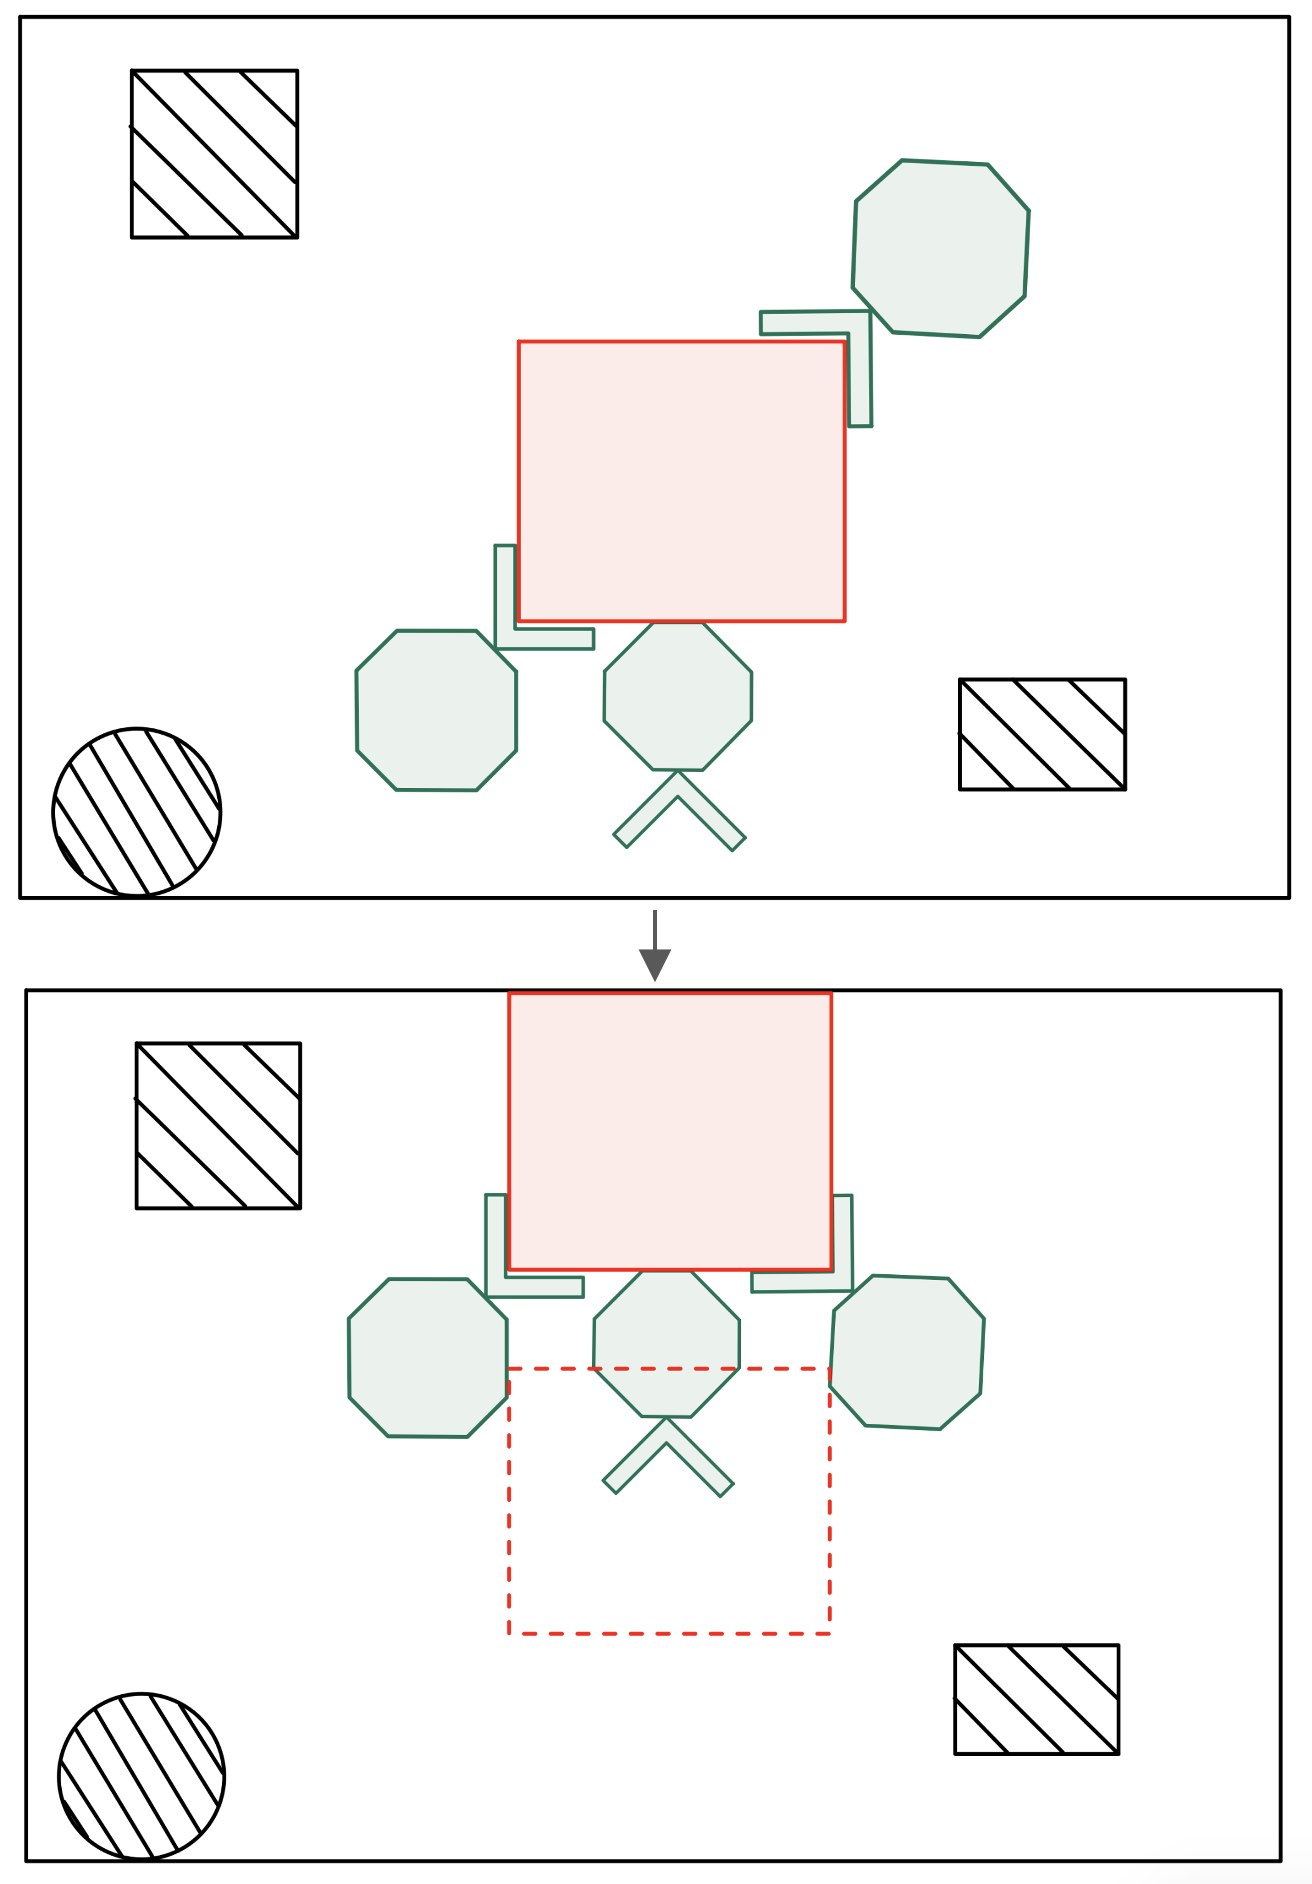
\includegraphics[width=0.75\linewidth]{assets/images/introduction/robot-transport-draw.png}
    \caption{Illustration of the project's goal: three robots transporting an object using a drawing}
    \label{fig:robot-transport-draw}
\end{figure}

\begin{figure} [H]
    \centering
    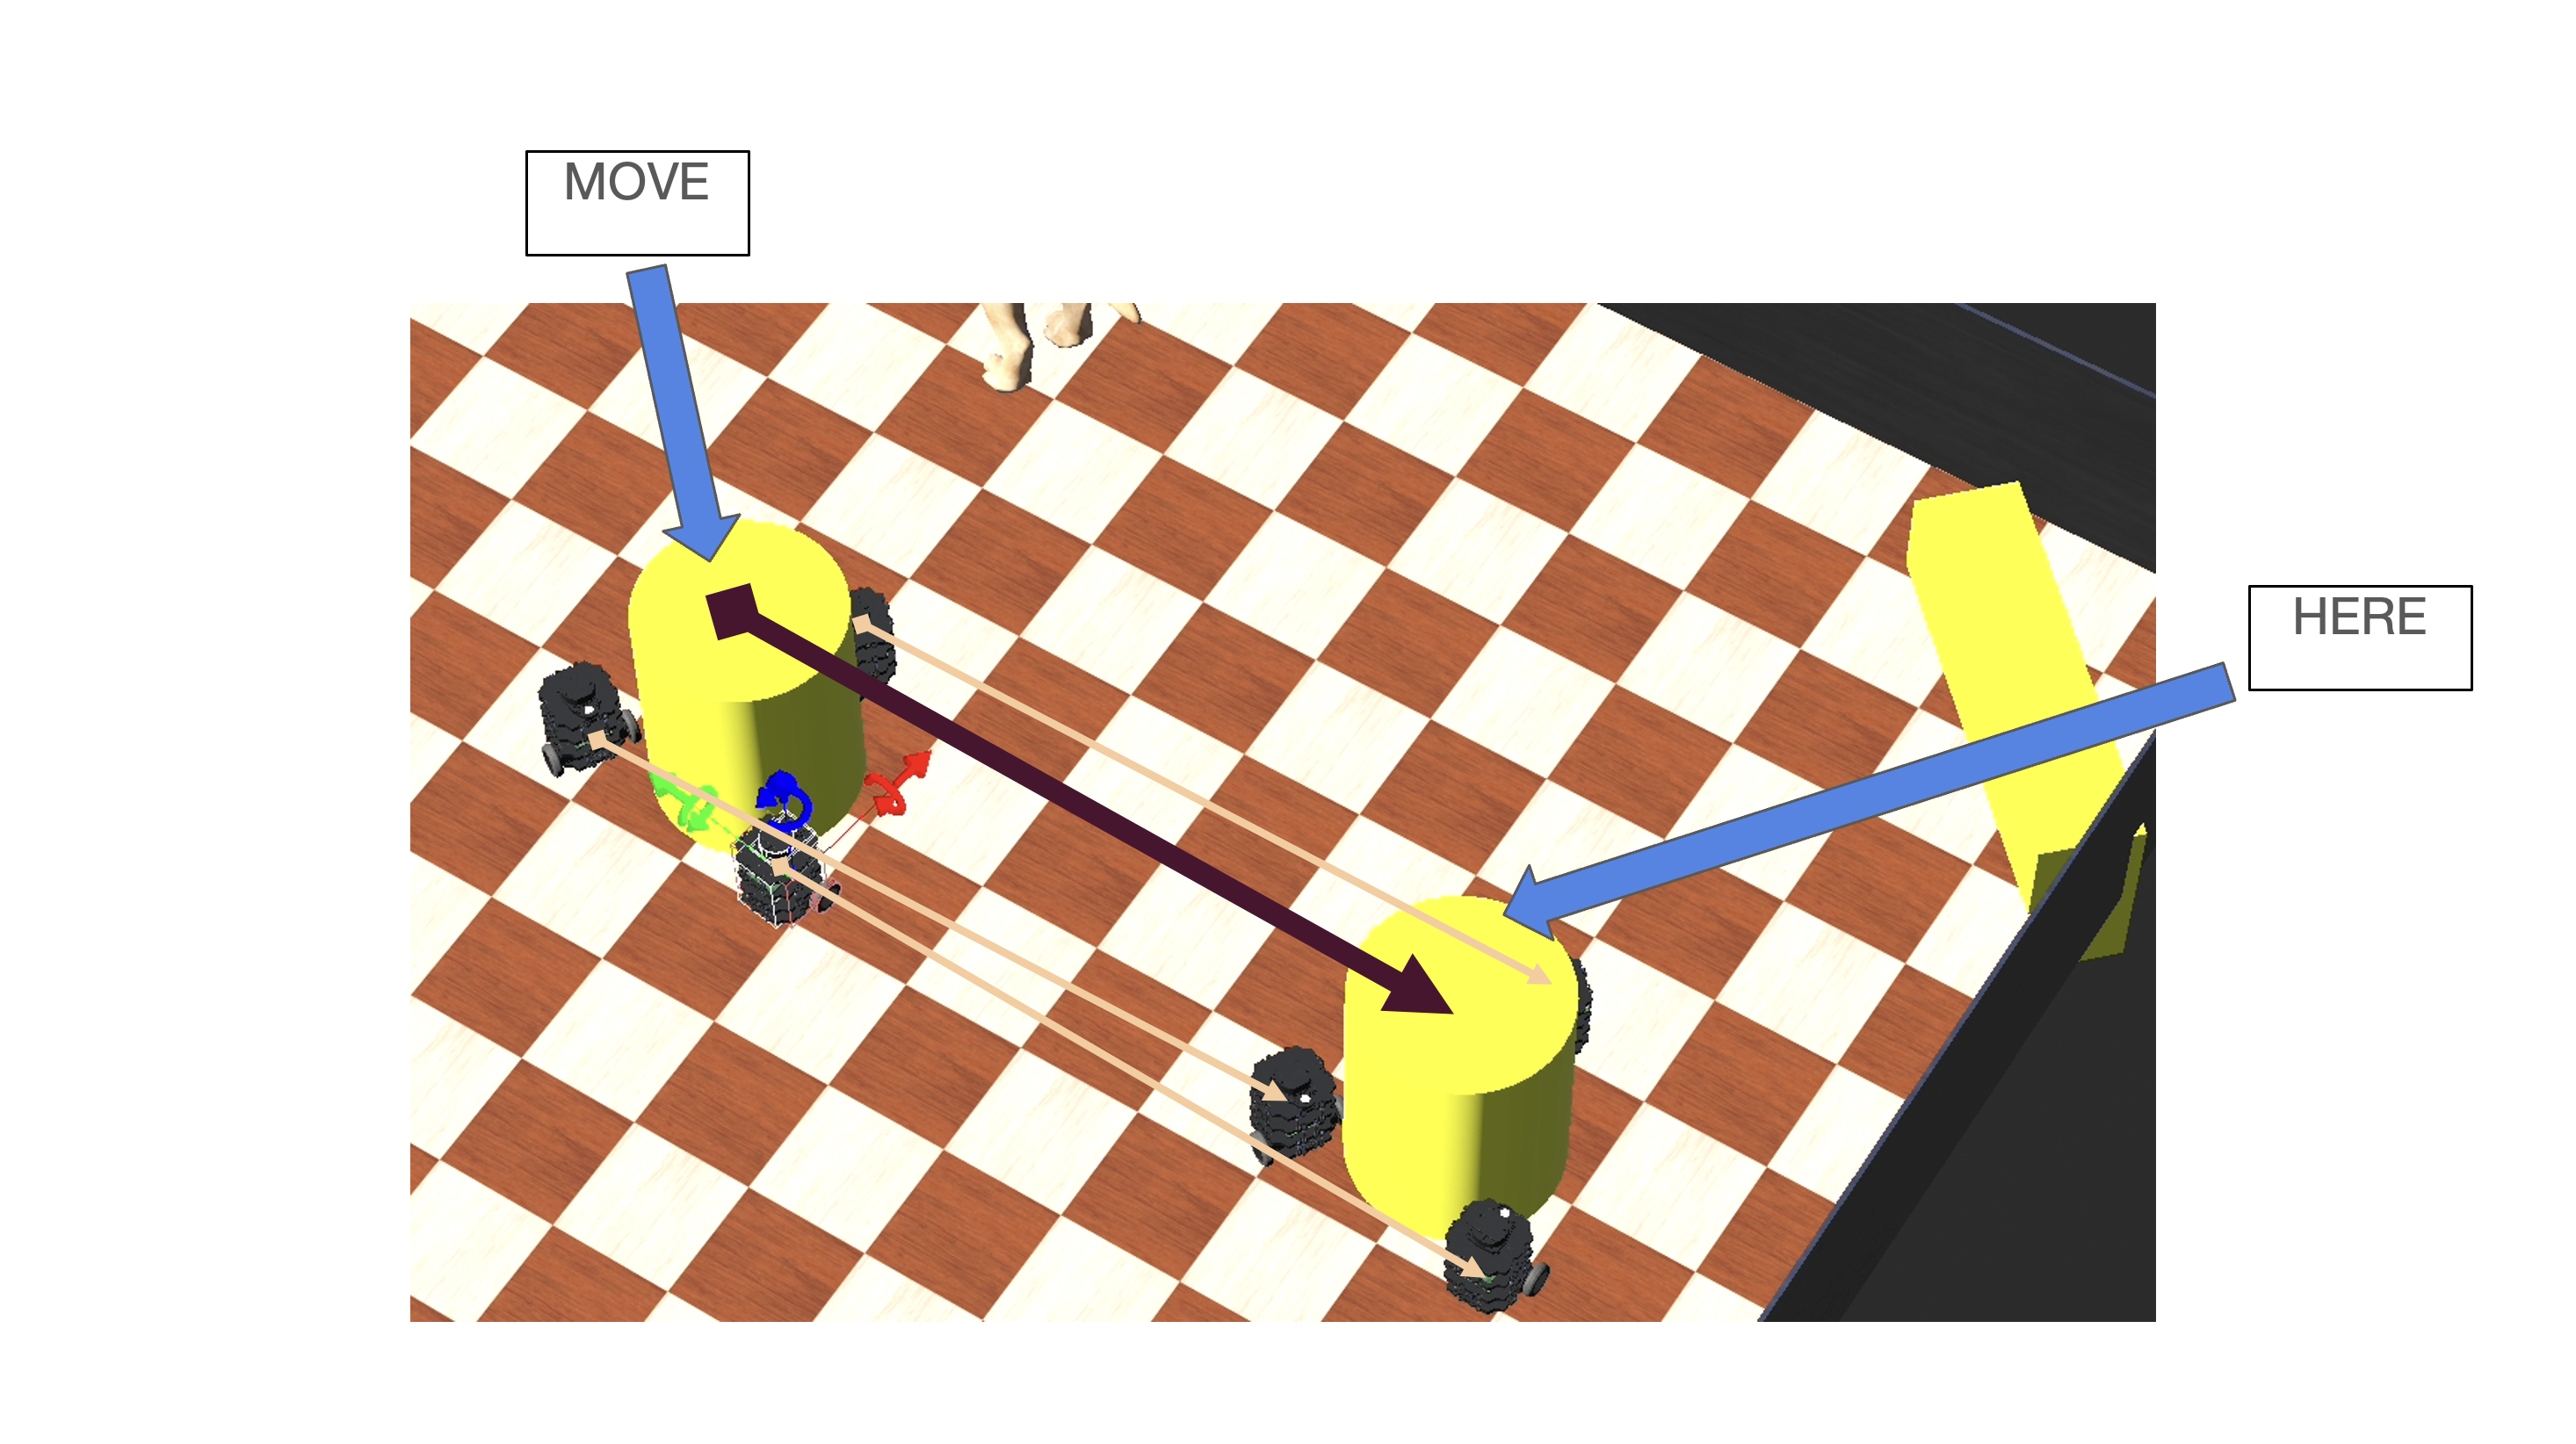
\includegraphics[width=1.0\linewidth]{assets/images/introduction/robot-transport-sim.png}
    \caption{Illustration of the project's goal: three robots transporting an object using simulation}
    \label{fig:robot-transport-sim}
\end{figure}

\paragraph*{}
A core objective of the project is to develop a system where three robots can simultaneously map their environment, communicate with one another, and collaborate to transport an object from point A to point B in a synchronised manner. This involves the robots autonomously detecting an object, localising themselves in the environment, and coordinating their movements to ensure seamless and efficient transport. This goal demonstrates the potential of decentralised swarm robotics for highly coordinated tasks that require precise communication and execution. See Figure \ref{fig:robot-transport-sim} for an simulation of the project's goal using the simulation.
See Figure \ref{fig:robot-transport-draw} for an illustration of the project's goal using a drawing 

\paragraph*{}
In real-world applications, this approach holds transformative potential, particularly in warehouse logistics and search-and-rescue operations. The decentralised model offers resilience and adaptability, making it suitable for scenarios where centralised systems may falter. Moreover, this technology aligns with Thailand’s growing need for innovative solutions in robotics, showcasing a shift towards decentralised systems that can operate independently without a centralised power hub. This represents a vision for the future of robotics, where hardware and computation costs decrease, enabling accessible and scalable robotic systems.

\paragraph*{}
The project development is divided into two phases:

\begin{enumerate}
    \item Phase 1: Exploration of foundational modules, including communication protocols, object detection via computer vision, and localisation. While the original plan included SLAM, it was deprioritised due to its limited necessity in the simulation phase.  A significant focus was placed on ensuring the robustness of these individual modules, validated through simulations in Webots, which provided a cost-efficient, risk-free environment.
    \item Phase 2: Integration of these foundational modules into a working prototype of robots navigating their environment. This phase also incorporates initial hardware configurations and an overhead camera to provide accurate odometry information for the robots. The ultimate goal is to transition from simulation to real-world applications, with the simulation results guiding the hardware design.
\end{enumerate}

\begin{figure} [H]
    \centering    
    \hspace*{-10cm} % adjust this value to suit your layo
    \vspace*{-0.8cm} % adjust this value to suit your layo
    
    \includegraphics[width=1.65\linewidth, angle=+90]{assets/images/introduction/flow-drawio-hi-res.png}
    \caption{High Level Flow Diagram of the project}
    \label{fig:high-level-flow}
\end{figure}



\paragraph*{}
The high level flowchat above is a detailed look at how different modules of our project come together. More details on each module will be expanded on later.
\paragraph*{}
The success of the project is measured not only by the accuracy and control of individual robots but also by the robustness of their communication and coordination. Metrics include the ability to resolve edge conditions, such as simultaneous object detection or potential collision paths, and the effectiveness of decentralised decision-making. Overhead cameras verify the robots’ positional accuracy, ensuring that simulated and real-world performance align

\paragraph*{}
This report highlights the project’s accomplishments, including completed tasks like communication, object detection, and localisation, alongside the progress of module integration. It also underscores the importance of simulation as a foundation for hardware development and presents a roadmap for achieving decentralised, collaborative transport systems. Through this effort, the project aims to establish a framework that not only advances robotics technology but also addresses challenges specific to Thailand, paving the way for future innovations in swarm robotics.

% ===== EDIT ABOVE PLEASE ===== %
\paragraph*{}
Building on the progress achieved in the previous semester, we successfully developed a Minimum Viable Prototype (MVP) of a swarm collective movement system within a simulated environment. This accomplishment sets the foundation for the current semester, where our initial focus is on preparing for the hardware implementation phase. Subsequently, we aim to realize our proposed concept through deployment on a physical swarm system, transitioning this towards the real-world implementation.

\paragraph*{}
This final report aims to highlight the progress of our project throughout the whole semester, with the evaluating criteria being the team's contributions alongside the pace in comparison to the ideal schedule. The ideal project timeline is presented with the Gantt Chart below. (Figure \ref{fig:gantt-chart})

\begin{figure} [H]
    \centering
    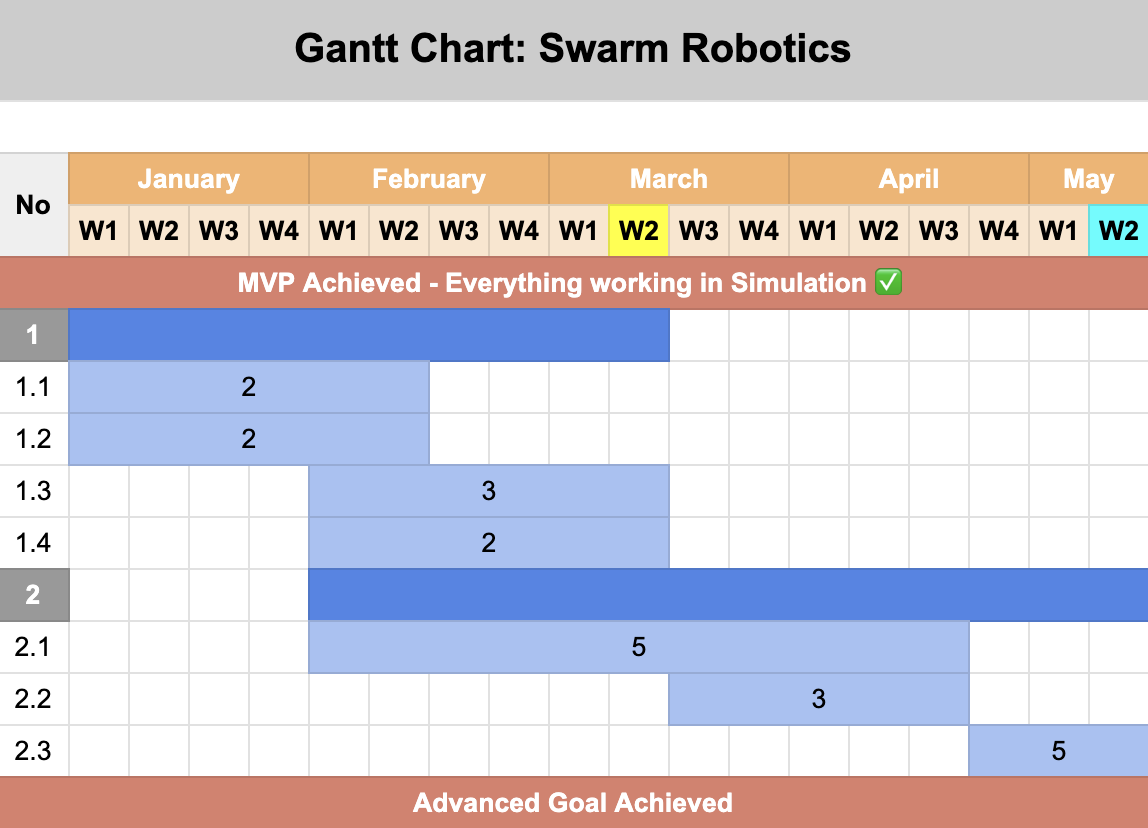
\includegraphics[width=1\linewidth]{assets/images/timeline/gantt_chart.png}
    \caption{Project Gantt Chart}
    \label{fig:gantt-chart}
\end{figure}

\paragraph*{Current Gantt Chart and Progress:}
\begin{description}
    \item[Phase 1: Preparation for Hardware Implementation]
    
    \item 1.1. Communication in the Swarm -- \textit{Completed} -- 
    Achieved communication in the swarm by using socket communication in a peer-to-peer architecture, alongside a consensus algorithm to handle communicatory conflicts

    \item 1.2. SLAM in Simulation -- \textit{Status} -- 
    Placeholder for details

    \item 1.3. Coordination and Formation -- \textit{Completed} --
    Enabled collisionless, planned movement towards a coordinated formation using waypoints, forming an equilateral formation around the detected target

    \item 1.4. Object Detection -- \textit{Completed} -- 
    Measure relative distance, relative angle, and diameter of the detected cylinder using multi-sensors fusion; camera and S3 RPLiDAR

    \item[Phase 2: Moving Towards a Complete Swarm]

    \item 2.1. Hardware -- \textit{Status} --
    Placeholder for details

    \item 2.2. Movement after Gripping -- \textit{Aborted} --
    Placeholder for details

    \item 2.3. Testing and Evaluation -- \textit{Status} -- 
    Placeholder for details
\end{description}
